\documentclass{report}

\usepackage{enumerate,fullpage,graphicx,hyperref}

\title{Emergent Architertural Design}
\date{Last edited: \today}
\author{Project members: \\
	Derk-Jan Karrenbeld - 4021967\\
	Joost Verdoorn - 1545396\\
	Steffan Sluis - 4088816\\
	Tung Phan - 4004868\\
	Vincent Robbemond - 4174097
	}

\begin{document}
	\maketitle

	\pdfbookmark{\contentsname}{toc}
	\tableofcontents

	\clearpage

	\setcounter{section}{0}
	\renewcommand*\thesection{\arabic{section}}
	
	\section{Introduction}
		This document contains the architectural design for the application created during the Context Project `Programming Life: Synthetic Biology'. The application is targeted at synthetic biologists and its main purpose is to easily model the complex workings of a cell. \\
		The design of this application is explained first in terms of its design goals. Then a subsystem decomposition follows, which serves to uncover the inner workings of the application, along with a description of the mapping of subsystems to processes and computers, a hardware/software mapping. After this, the management of data and shared resources is discussed. In conclusion a short summary of the system architecture is given.
		\subsection{Design goals}
			Because the application has a very specific use, modelling cells and the processes within, the main design goal is to make this as easy and intuitive as possible. Secondary to this goal is the possibility to access the application from every common platform, such as not only desktop and laptop, but also mobile devices. Of course, working and optimally performing software is the first goal to be strived towards.
			Because the field of technology this application targets is fairly new, another design goal is to meet this field by using new technologies. The teammembers actively agreed that they want to innovate and do selfstudy to broaden their knowledge. 
			Lastly, the software that is being developed should by maintainable. 
	\clearpage
	\section{Software architecture views}
		This section contains all the information about the software architecture of the application. The section is divided into several subsections to group together interesting information and improve readability.
		\subsection{Subsystem Decomposition}
			This section describes the key subsystems in the application. It is divided into two sections, because the application is diveded this way as well. The first subsection is about the server-side subsystems and the second one is about the client-side subsystems.
			\subsubsection{Server side}
				The server subsystems consist of two key parts: the server backend and the database. The server keeps an up to date copy of the database and sychronises with the client side when possible. It can also be used to do calculations that are too complicated for the client-side of the application. It is dependent upon the database, to synchronize the appropriate data to the appropriate client-backend corresponding with a user.
				The database is used for storage of user data, modules for cell design, as well as cell models created using the application. It provides a centralized storage so the client-side application can function on any platform without a persistent internet connection. It is not dependent upon anything, although every function used persistent data is dependent on it. 
				A certain number of technologies are involved in the serverside.
				\subsubsubsection{Rails}
					The server runs on Ruby on Rails. This is a fairly new but very stable platform that is not only free but also open source. This means active development by a lot of people. Problems are easily fixed and this should ease the use of the application that is being designed. The language itself is written from a standpoint where you should just be able to write code and not worry about breaking the interpreter. This makes it easy to write complex code.
				\subsubsubsection{MVC}
					The pages served are HTML5 for markup with CSS3 for styling and Javascript for interaction. Pages are built by a comprehensive and solid Model-Viewer-Controller system. This keeps data separated from the representation, further increasing maintainability. 
				\subsubsubsection{Models and Database}
					Ruby models are mapped to any SQL enabled language such as SQLLite, MySQL and PostgreSQL. By not restricting the server database technology, switching systems, servers or extending  their capacity should be fairly simple and easy.
				\subsubsubsection{Views and ERB}
					The views are in ERB which is an HTML template system. It is provided with the default Ruby library, so it does not require any extra software. Ruby controllers can expose data to these views. New views are easily added this way, so new ways of data representation are quickly devised.
				\subsubsubsection{Coffeescript and Javascript}
					Interaction assets are written in Coffeescript, which is a language specially designed to make Javascript more maintainable, readable and cleaner alltogether. Coffedoc is used to document this code and Jasmine is used to test the javascript output. In production a script called uglifier minifies and bundles all the scripts.
				\subsubsubsection{SASS and CSS}
					Styling assets are written in a language called Syntactically Awesome Stylesheets. Similar to CoffeeScript, SASS makes it easier and cleaner to create extensive CSS. 
			\subsubsection{Client side}
				The client side subsystems contain most of the applications functionality. These subsystems are responsible for displaying the graphical environment with all it's modules, as well as doing the basic simulating. If the simulation becomes too complex, the complicated calculations can be sent to the sever to be processed on the server side. If used locally, the client side subsystems function independently of the server. If used on multiple machines, the client side can be made dependent on the server and the database to synchronize user data.
				\subsubsubsection{Localstorage}
					Javascript determines the local storage engine that is avaialbe and uses that to maintain an offline copy of the application. This makes it very easy to design new cells. 
				\subsubsubsection{Interaction by Javascript}
					Javascript facilitates interaction and processes all the differential equations. It generates the graphs and the reports. 
		\subsection{Hardware/software mapping}
			The hardware/software mapping is illustrated by the image below. The server is a non-client piece of hardware, and can therefore be chosen specifically to suit the clients needs. The client side hardware is required to support current webbuilding standards, which qualifies almost every machine from almost every platform to run the application.\\
			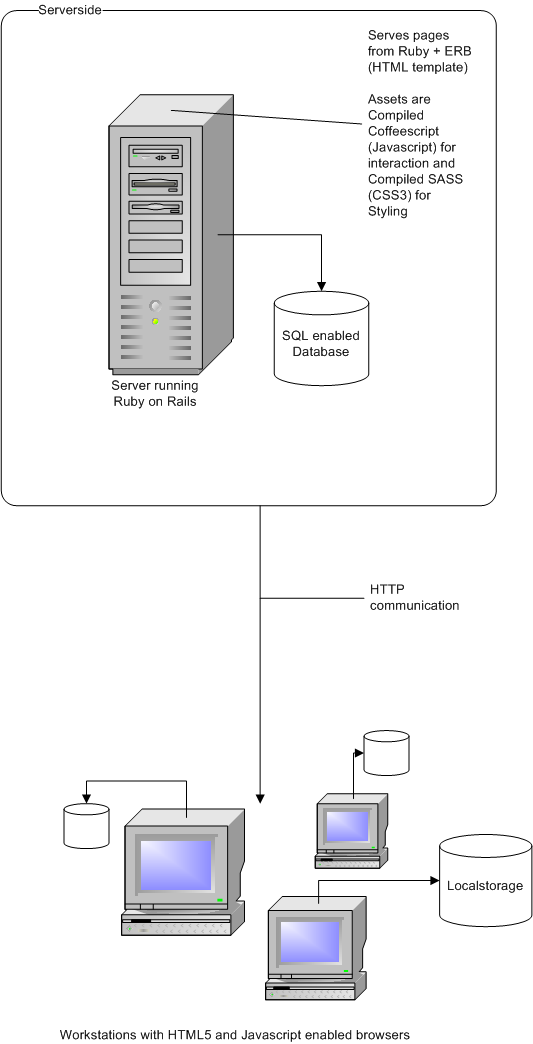
\includegraphics[width=16cm]{EAD.png}
		\subsection{Persistent data management}
			The application synchronizes any persistent data with the database running on the server. This ensures availability of all user data if there is a connection to the server. The application also provides the possibility to store data locally and export simulation results to a report in multiple standardized format, such as \emph{HTML}, \emph{Excel} and \emph{PDF}.			
		\subsection{Concurrency}
			Each client runs independently and used asynchronous communication with the server through \emph{REST} and \emph{AJAX}. Because of this, concurrency issues are very improbable. The client side application is web-based, and uses only one process. Shared resources are retrieved directly from and synchronized directly with the database.
	\clearpage
	\section{Summary}
		The application is a lightweight, cross-platform graphical design tool with a centralized storage database. The architecture ensures it's functionality on different kinds of machines as well as the ease of simulating complex cell models. It not only offers stability, ease and intuitive design, it offers it on every machine.
	\section{Glossary}
		This section explains any and all terms that may be ambiguous or unclear:\\
\end{document}
